\documentclass{beamer}

\usepackage{amssymb}
\usepackage{fancyvrb}
\usepackage{stmaryrd}
\usepackage{graphicx}
\usefonttheme{serif}


\newcommand{\Nat}{\mathbb{N}}

\title{Compilers}%\texorpdfstring{$\mathbb{N}$}}
\subtitle{CMSC 430}
\date{January 28\textsuperscript{th}, 2020}

\usetheme{jmct}

\usepackage{calc}

\newcommand{\textover}[3][l]{%
 % #1 is the alignment, default l
 % #2 is the text to be printed
 % #3 is the text for setting the width
 \makebox[\widthof{#3}][#1]{#2}%
 }

\newcommand{\blueit}[1]{%
  {\color{dark-lucid-blue}#1}%
}
\newcommand{\blueite}[1]{%
  \blueit{\emph{#1}}%
}


\newcommand{\myquote}[3]{
  ``#1''
  \vspace{3pt}
  \hrule
  \begin{flushright}
  --- \blueit{\emph{#2}}, \emph{#3}
  \end{flushright}
}

\begin{document}
	\frame {
		\titlepage
	}

%%%%%%%%%%%%%%%%%%%%%%%%%%%%%%%%%%%%%%%% 
%%% Intro
%%%%%%%%%%%%%%%%%%%%%%%%%%%%%%%%%%%%%%%% 

  \frame{
    \frametitle{This Lecture}
    What is a compiler?
  }

  \frame{
    \frametitle{Before we start...}
      \begin{enumerate}
        \item<2 - 4> Who am I?
        \item<3 - 4> Who are the TAs?
        \item<4 - 4> Some admin
      \end{enumerate}
  }

  \frame{
    \frametitle{Who am I?}
      \onslide<2>{Research Scientist at a research services firm}

      \onslide<3>{PhD in Compilers}

      \onslide<4>{BS Music Engineering}
  }

  \frame{
    \frametitle{Who are the TAs?}
    \onslide<2>{\begin{itemize}
      \item Sankha Narayan Guria
      \item Tasnim Kabir
      \item Ivan Quiles-Rodriguez
      \item John Kastner
      \item Yiyun Liu
    \end{itemize}
    }
  }

  % Here is where I apologize for not having UMD credentials
  \frame{
    \frametitle{Adminapology}
  }

%%%%%%%%%%%%%%%%%%%%%%%%%%%%%%%%%%%%%%%% 
%%% What is a Compiler
%%%%%%%%%%%%%%%%%%%%%%%%%%%%%%%%%%%%%%%% 

  \frame{
    \frametitle{\blueite{What} is a compiler?}
    \onslide<2>{If I've done my job right: Everything.}

    \onslide<3>{Compilers are everwhere, as compiler-writers this is a blessing and a curse.}

    \onslide<4>{I will always have a job, if I want it.}

  }

  \frame{
    \frametitle{Compilers are \blueite{everywhere}}
    \onslide<2->{I have seen compilers on:}
    \begin{itemize}
      \item<3-> Phones
      \item<4-> Printers
      \item<5-> SmartCards
      \item<6-> Space Stuff (NASA Deep Space 1)
      \item<7-> Scariest of all:
      \begin{itemize}
        \item<8-> The Linux Kernel itself
      \end{itemize}
    \end{itemize}
  }

  \begin{frame}[fragile]
    \frametitle{What is a \blueite{compiler}?}
    \begin{itemize}
      \item<1-> Easy:
      \begin{itemize}
        \item<2 -> {\color{dark-gray} \verb`compiler : SourceProgram -> TargetProgram`}
      \end{itemize}
    \end{itemize}
  \end{frame}

  \begin{frame}[fragile]
    \frametitle{Source Programs}
    \begin{itemize}
      \item<2-> Concrete Syntax
      \item<3-> Parsers
      \item<4-> Grammars (LR, LALR, GLR, etc.)
      \item<5-> i.e. "what the programmer writes"
    \end{itemize}
  \end{frame}

  \begin{frame}[fragile]
    \frametitle{Target Programs}
    \onslide<2> Could be anything, but...

    \onslide<3-> Often:
    \begin{itemize}
      \item<3-> Machine Code
      \item<4-> Byte Code
      \item<5-> Another Programming Language (i.e. C to Javescript)
      \item<6-> Information/Data for tooling
    \end{itemize}
  \end{frame}

  \frame{
    \frametitle{Show me}
    \begin{figure}
      \centering
      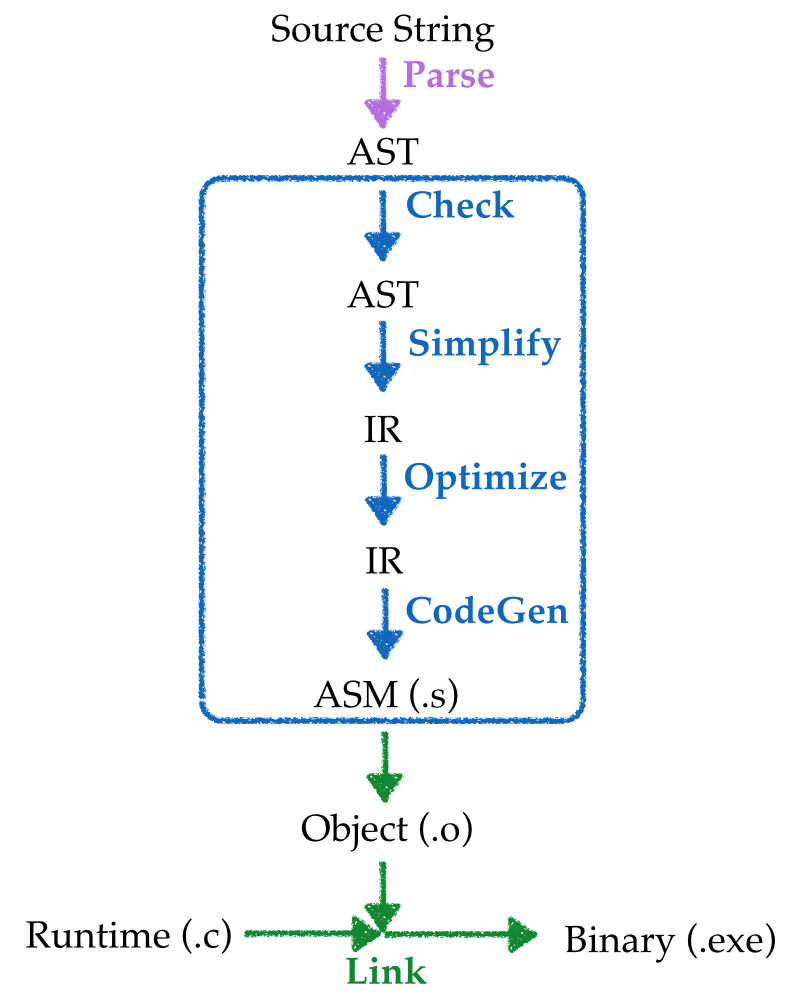
\includegraphics[height=0.75\textheight]{../img/compiler-pipeline.png}
    \end{figure}
  }

  \frame{
    \frametitle{It's a convenient lie}
    \onslide<2-4> {Compilers don't always have that form.}
    \onslide<3-4> {In fact, it is increasingly rare that they do!}

    \onslide<4> {\bigskip Regardless, it's a useful \emph{intuition} and allows us
      to cover all the important concepts.}

    \onslide<5> {Can anyone think of when a compiler \blueite{does not} have that form?}
  }

  \frame{
    \frametitle{What's important about the Souce-Target relationship?}
    \onslide<2> {Put another way: When you \blueite{write} a program, what do you expect
    the implementation of the programming language to do (or not do)?}
  }


%%%%%%%%%%%%%%%%%%%%%%%%%%%%%%%%%%%%%%%% 
%%% This Class
%%%%%%%%%%%%%%%%%%%%%%%%%%%%%%%%%%%%%%%% 

  \frame{
    \frametitle{This class}
    \onslide<2-> {CMSC 430 is about the study of that relationship. In particular:}
    \begin{itemize}
      \item<3-> How do we bridge the gap between `high-level' and `low-level' languages?
        \begin{itemize}
          \item<4,5> CMSC 330: `high-level'
          \item<5> CMSC 216: `low-level'
        \end{itemize}
      \item<6-> What does it \blueite{mean} to bridge that gap?
        \begin{itemize}
          \item<7> Do \emph{all} the features of one language need to be present in the other?
        \end{itemize}
      \item<8> In other words: This class is about \blueite{abstraction}.
    \end{itemize}
  }

  \begin{frame}[fragile]
    \frametitle{The result}
    \begin{itemize}
      \item<2-> Goal is to write a compiler for {\color{dark-gray} \verb`NanoML -> X86`}
      \item<3-> This includes looking at
        \begin{itemize}
          \item<4-> Parsing
          \item<5-> Checking and Validation
          \item<6-> Simplification and Normalization (sometimes known as \emph{Elaboration})
          \item<7-> Optimization
          \item<8-> Code Generation
        \end{itemize}
    \end{itemize}
  \end{frame}

  \frame{
    \frametitle{Why is this interesting?}
    \onslide<2-> {I find compilers/interpreters/PLs interesting in their own right, but
    not everyone shares the same aesthetic values.}
    \begin{itemize}
      \item<3-> Compilers combine several important aspects of CS
        \begin{itemize}
          \item<4,5> Theory (parsing, types, ASTs, semantics, etc.)
          \item<5> Systems (computer architectures, performance, sys-calls, etc.)
        \end{itemize}
      \item<6-> Unlike some other major software artifacts, compilers \emph{can be} well specified!
        \begin{itemize}
          \item<7> This lets us reason about \blueite{correctness}
        \end{itemize}
      \item<8> Develop good habits on non-trivial software projects.
    \end{itemize}
  }

  \frame{
    \frametitle{Most important point of the day}
    \onslide<2> {The `dragon book' lied.}
    \onslide<3-> {Compilers are not scary.}
  }

  \frame{
    \frametitle{How we'll do it}
    \onslide<2-> {We will write \emph{several} compilers.}

    \onslide<3-> {Each will be simple and implement a specific feature or set of related features.}

    \onslide<4-> {Combining these compilers is what gives us powerful abstractions.}
  }


%%%%%%%%%%%%%%%%%%%%%%%%%%%%%%%%%%%%%%%% 
%%% Conclusion
%%%%%%%%%%%%%%%%%%%%%%%%%%%%%%%%%%%%%%%% 

  \frame{
    \frametitle{Any Questions?}
  }

  \frame{
    \frametitle{Closing thoughts}
    \onslide<2> {Please read over the syllabus on the website and reach out to
      me if there are any issues.}
  }

  \frame{
    \frametitle{}
    Thanks for your time!

  }

\end{document}
